\subsection{Effect of different codebook sizes}
The effect of changing the size of the codebook is shown in table \ref{tab:clusters} and figure \ref{plot:codebook}. In general, a smaller codebook performs better than a large codebook due to the data tending to overfit when a large codebook is used. However, the codebook is too small (e.g. 100 codewords), it is unable to capture enough detail to properly disambiguate classes. The tipping point for the best performance regarding the codebook size is 200.

\begin{figure}[H]
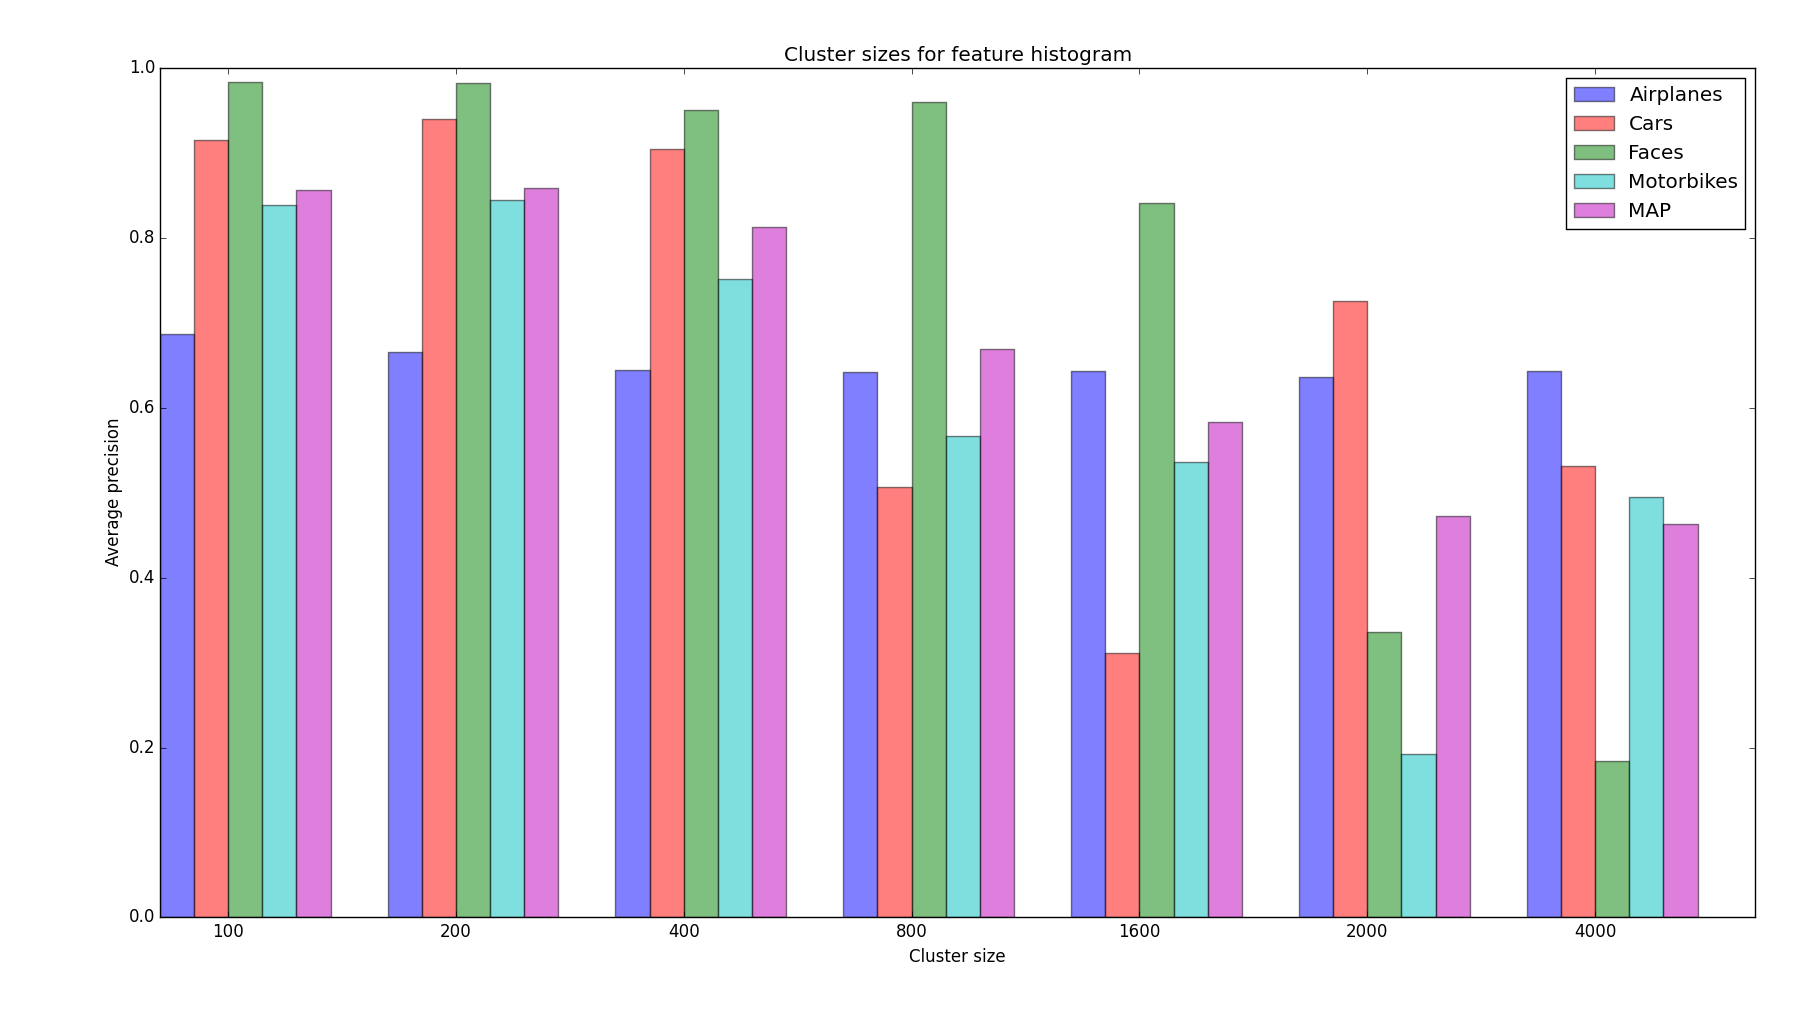
\includegraphics[width=\textwidth]{../plots/cluster_size_feature_histograms}
\caption{Effect of codebook size on AP}
\label{plot:codebook}
\end{figure}
\begin{table}[H]
\begin{center}
\begin{tabular}{|c|ccccc|}
\hline
\textbf{Codebook size} & \textbf{AP Airplanes} & \textbf{AP Cars} & \textbf{AP Faces} & \textbf{AP Motorbikes} & \textbf{MAP}\\
\hline
100& 0.6868 & 0.9152 & 0.9843 & 0.8395 & 0.8564\\
200 & 0.6663 & 0.9408 & 0.9824 & 0.8454 & 0.8587\\
400 & 0.6447 & 0.9053 & 0.9510 & 0.7516 & 0.8132\\
800 & 0.6424 & 0.5067 & 0.9602 & 0.5667 & 0.6690\\
1600 & 0.6438 & 0.3115 & 0.8410 & 0.5361 & 0.5831\\
2000 & 0.6367 & 0.7253 & 0.3357 & 0.1926 & 0.4726\\
4000 & 0.6430 & 0.5311 & 0.1837 & 0.4956 & 0.4634\\
\hline
\end{tabular}
\caption{Effect of different codebook sizes, Sift type: dense, Color space: opponent}
\label{tab:clusters}
\end{center}
\end{table}
